\documentclass[12pt,a4paper]{article}
\usepackage[utf8]{inputenc}
\usepackage[T1]{fontenc}
\usepackage{amsmath}
\usepackage{amssymb}
\usepackage{graphicx}
\usepackage[left=2.00cm, right=2.00cm, top=2.00cm, bottom=2.00cm]{geometry}
\usepackage{hyperref}

\usepackage{setspace}
\usepackage{siunitx}
\DeclareSIUnit\rydberg{Ry}
\usepackage{tikz}
\usepackage{paralist}
\usepackage[version=4]{mhchem}
\usepackage{booktabs}
\usepackage{rotating}
\usepackage{chngcntr}

\title{Prediction of XPS binding energies for molecules grafted on calcium surfaces}
\author{Pierre Beaujean}
\date{Version of \today}

\allowdisplaybreaks
\onehalfspacing

\def\dbe{\ensuremath{\Delta\text{BE}}}

\begin{document}
\maketitle

\section{Introduction}

Batteries are one of the key enabling technologies for transitioning to a climate-neutral society. Since their market introduction, lithium-ion batteries (LIBs) have developed into a very mature technology and are currently used in numerous applications. However, despite their established performance, LIBs are unlikely to meet the foreseen objectives required for large-scale applications due to three key issues:
\begin{inparaenum}[(i)]
	\item availability of raw materials (currently involving rare-earth metals),
	\item low energetic density, and
	\item poor sustainability over a large number of cycles.
\end{inparaenum}

The ECOBAT project aims to address the second point by using divalent cations, such as \ce{Ca^2+}. However, due to its high reactivity, specially designed electrolytes are required to achieve a reversible mechanism. Understanding the chemistry of its solid-electrolyte interphase (SEI) is also crucial.

In the literature, calcium batteries (CIBs) use carbonate-containing electrolytes such as dimethyl ether (DME), ethylene carbonate (EC), glyme, or tetrahydrofuran (THF), mixed with weakly coordinated anions such as \ce{BH4-} or \ce{BF4-} \cite{zhaoRevealingSolidElectrolyte2022,taghavi-kahaghPoweringFutureComprehensive2023}. While there are experimental \cite{melemedImpactDifferentialCa22023} and theoretical \cite{hahnCriticalRoleConfigurational2020,liepinyaComputationalComparisonEther2021,pathreekerWhyTetrahydrofuranGood2021,yamijalaStabilityCalciumIon2021} studies on SEI formation, a better understanding can be achieved by combining experimental spectra with theoretical calculations using spectroscopic tools.

X-ray photoelectron spectroscopy (XPS) is a surface-sensitive, quantitative spectroscopy that allows for the identification of elements within the material or at its surface. It belongs to the family of photoemission spectroscopies, where the energy of electrons emitted by the photoelectric effect is analyzed. Specifically, XPS uses a beam of soft X-rays (\SI{100}{\electronvolt} < $h\nu$ < \SI{10}{\kilo\electronvolt}), enabling the probing of core electrons (low principal quantum number) \cite{stevieIntroductionXrayPhotoelectron2020}. It is routinely used to gain understanding of SEI composition, both experimentally \cite{melemedImpactDifferentialCa22023} and theoretically \cite{ebadiInsightsLiMetalOrganic2019}.

This study focuses on the XPS spectra resulting from the degradation of THF as a model system. Different possible degradation products (Fig.~\ref{fig:THFdegradation}) will be considered on various calcium substrates, including calcium oxide and hydride.

\begin{figure}
	\centering
	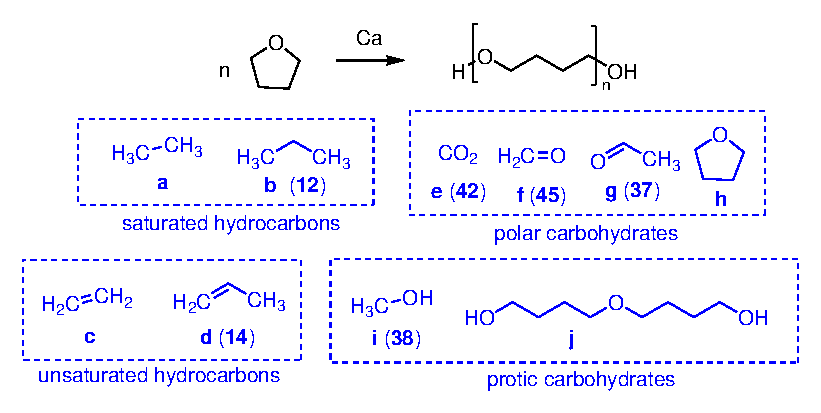
\includegraphics{Figure1}
	\caption{The main degradation pathway of THF leads to THF polymer (black). Compound \textbf{a}-\textbf{i} (blue) are considered in this study: \textbf{a} is used as a model for the THF polymer, while fragmentation may lead to (un)saturated hydrocarbons (\textbf{b}-\textbf{e}) or carbonates (\textbf{f}-\textbf{i}).}
	\label{fig:THFdegradation}
\end{figure}

\section{Theoretical methods}

In XPS spectroscopy, the conservation of energy is described by the equation:
\begin{equation}
	h\nu = \text{BE} + E_{\text{kin}} + \phi, \label{eq:xps}
\end{equation}
where BE is the binding energy of the electron, $E_{\text{kin}}$ is the kinetic energy of the emitted electron (measured by the detector), and $\phi$ is the work function, which accounts for surface effects and detector contributions. Using a source of monochromatic X-rays (such as Al $K_\alpha$, $h\nu = \SI{1486.7}{\electronvolt}$), it is possible to determine BE from $E_{\text{kin}}$ \cite{vinesPredictionCoreLevel2018}. The binding energy depends on how tightly the electron is bound to its orbital, making it sensitive to the oxidation state and chemical environment of the originating atom. Generally, more electronegative surroundings result in higher BE, providing information on the atom's environment, much like chemical shifts in NMR.

From a quantum chemistry perspective, binding energy is akin to the ionization energy of core electrons:
\begin{equation}
	\text{BE}_i = E^{N-1}_i(\text{final}) - E^{N}(\text{initial}), \label{eq:dscf}
\end{equation}
where $E^{N}$ and $E^{N-1}$ are the energies of the initial $N$-electron non-ionized state and the final $N-1$ electron ionized state with a core hole on atom $i$. While these energies could be obtained through (relativistic) multi-configuration approaches, this is impractical for large systems. Even CIS or TD excitations are challenging to target, as they correspond to highly excited states \cite{vinesPredictionCoreLevel2018}.

For gas-phase molecules, classical quantum chemistry tools can be utilized. At the HF level, core-level BE can be approximated using Koopmans' theorem, which correlates to the orbital energy of the removed electron. This is known as the initial state (IS) or frozen orbitals (FO) approach. However, relaxation effects are neglected. More accurate values can be obtained using Eq.~\eqref{eq:dscf}, by computing the energy difference between initial and final states at the HF level, known as the $\Delta$SCF approach, which includes final state (FS) effects. While this method may provide quantitative agreement in some cases, electron correlation effects are significant, necessitating the use of density functional theory (DFT), for which Koopmans' theorem no longer applies \cite{pueyobellafontPredictingCoreLevel2017}.

Treating solids or surfaces adds complexity. Generally, only valence levels are explicitly treated, with pseudopotentials (PPs) modeling core electrons. The projected augmented wave (PAW) method maps results to all-electron wave functions using specially designed PPs and transformations \cite{blochlProjectorAugmentedwaveMethod1994}. In codes like CP2K or VASP, a core hole can be generated, neglecting the relaxation of other core electrons but including valence electron relaxation. This limits the accuracy of absolute BE descriptions.

Another challenge arises with periodic boundary conditions, where the core hole is periodically repeated, creating an infinitely charged system. Two approaches can address this: 
\begin{inparaenum}[a)]
	\item add the excited electron to the bottom of the conduction band (or LUMO for isolated molecules), or 
	\item remove the excited electron from the system and use a background counter-charge.
\end{inparaenum}
The first approach underestimates BEs, resembling absorption processes, while the second induces physically incorrect effects, further complicating absolute BE prediction.

However, relative BE can be estimated by computing wave functions for a fractional number of electrons using Slater transition state theory and Janak's theorem \cite{janakProofThatFrac1978}, resulting in the Slater-Janak (SJ) approach \cite{hiraoImprovedSlaterTransition2021}. In this work, BE are computed with a half-electron placed either in the conduction band or in the vacuum, referred to as the SJ and SJ\textsuperscript{n} approaches, respectively (Fig.~\ref{fig:method}).
	
	\begin{figure}[!h]
		\centering
		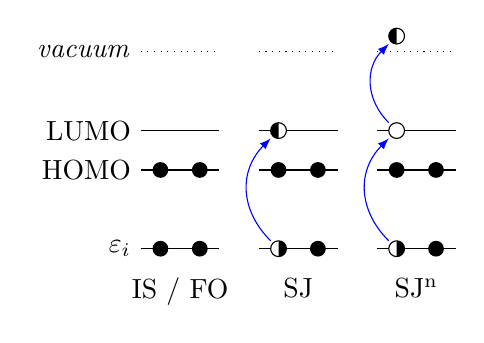
\begin{tikzpicture}
			\draw (0,0) node[left]{$\varepsilon_i$}-- node[midway,below=.25cm]{IS / FO} +(1,0);
			\draw (0,1) node[left]{HOMO}-- +(1,0);
			\draw (0,1.5) node[left]{LUMO}-- +(1,0);
			\draw[dotted] (0,2.5) node[left]{\textit{vacuum}}-- +(1,0);
			\fill (.25,0) circle (.1cm);
			\fill (.75,0) circle (.1cm);
			\fill (.25,1) circle (.1cm);
			\fill (.75,1) circle (.1cm);
			
			\begin{scope}[xshift=1.5cm]
				\draw (0,0) -- node[midway,below=.25cm]{SJ} +(1,0);
				\draw (0,1) -- +(1,0);
				\draw (0,1.5) -- +(1,0);
				\draw[dotted] (0,2.5) -- +(1,0);
				\draw[fill=white] (.25,0) circle (.1cm);
				\fill (.25,-.1) arc (-90:90:.1);
				\fill (.75,0) circle (.1cm);
				\fill (.25,1) circle (.1cm);
				\fill (.75,1) circle (.1cm);
				\draw[fill=white] (.25,1.5) circle (.1cm);
				\fill (.25,1.4) arc (-90:-270:.1);
				\draw[-latex,blue] (.15,.1) .. controls +(-.4,.4) and +(-.4,-.4) .. (.15,1.4);
			\end{scope}
			
			\begin{scope}[xshift=3cm]
				\draw (0,0) -- node[midway,below=.25cm]{SJ\textsuperscript{n}} +(1,0);
				\draw (0,1) -- +(1,0);
				\draw (0,1.5) -- +(1,0);
				\draw[dotted] (0,2.5) -- +(1,0);
				\draw[fill=white] (.25,0) circle (.1cm);
				\fill (.25,-.1) arc (-90:90:.1);
				\fill (.75,0) circle (.1cm);
				\fill (.25,1) circle (.1cm);
				\fill (.75,1) circle (.1cm);
				\draw[fill=white] (.25,1.5) circle (.1cm);
				\draw[-latex,blue] (.15,.1) .. controls +(-.4,.4) and +(-.4,-.4) .. (.15,1.4);
				\draw[-latex,blue] (.15,1.6) .. controls +(-.3,.3) and +(-.3,-.3) .. (.15,2.6);
				\draw[fill=white] (.25,2.7) circle (.1cm);
				\fill (.25,2.6) arc (-90:-270:.1);
			\end{scope}
		\end{tikzpicture}
		\caption{Approaches to compute BE as the energy of the molecular orbital where the core hole is located: initial state (IS, also referred to as frozen orbitals, FO) and Slater-Janak (SJ). When the electron is further removed from the system (and conceptually pushed to the vacuum), JS\textsuperscript{n} is noted. Adapted from Ref.~\cite{pueyobellafontPredictingCoreLevel2017}.}
		\label{fig:method}
	\end{figure}

Finally, while the determination of absolute binding energies (BE) is challenging from a theoretical perspective, the measurement or calculation of the work function, $\phi$ in Eq.~\eqref{eq:xps}, is also complex. As a result, both experimentalists and quantum chemists often focus on the relative binding energy, $\Delta\text{BE}$, which is the difference in binding energy for a given atom with respect to a reference compound \cite{vinesPredictionCoreLevel2018}. In this contribution, relative BE values are computed as $\Delta\text{BE}_i = \text{BE}_i - \text{BE}(\text{ref})$, using the calculated or experimental BE values for \ce{CH4}, \ce{NH3}, \ce{H2O}, \ce{B2H6}, and \ce{HF} as references for carbon, nitrogen, oxygen, boron, and fluorine, respectively. The experimental values are taken from Ref.~\cite{pueyobellafontPredictingCoreLevel2017}. For calcium, the innermost atom of a 1x1 Ca slab containing 16 layers is used as the reference.

	
\section{Computational details}

Unless otherwise stated, all calculations were performed using the PBE-D3 level of theory with VASP (version 6.4.1) and the projector-augmented wave (PAW) method \cite{blochlProjectorAugmentedwaveMethod1994}. The energy convergence criterion was set to \SI{e-4}{\electronvolt}, with a cutoff of \SI{550}{\electronvolt} for the kinetic energy of the plane waves. Gaussian smearing of the valence electrons, with a width of \SI{0.2}{\electronvolt}, was applied. Brillouin zone integration was performed at the gamma point for molecules in the gas phase, using a 4x4x4 Monkhorst-Pack k-point mesh for bulk calculations, and a 4x4x1 mesh for slab calculations. The \texttt{Ca\_sv} pseudopotential was employed to model calcium.

All optimizations were carried out using the L-BFGS algorithm, driven by ASE \cite{larsenAtomicSimulationEnvironment2017} with VASP energies and forces, until the force on all atoms was below \SI{e-2}{\electronvolt\per\angstrom}.\footnote{For IR spectroscopy, a target of \SI{e-3}{\electronvolt\per\angstrom} is required to avoid large (> \SI{1000}{\per\centi\meter}) imaginary frequencies.}

For the calculation of binding energies (BE), VASP allows targeting a specific orbital, $i$, from which a half-electron is removed. For SJ\textsuperscript{n}, it is also necessary to set the appropriate number of valence electrons using the \texttt{NELECT} keyword. After the calculation, the eigenvalue, $\varepsilon_i\left(\frac{1}{2}\right)$, is extracted. The binding energy is then computed as follows:
\begin{equation}
	\text{BE}_i = 	\begin{cases}
		-\varepsilon_i\left(\tfrac{1}{2}\right) & \text{if gas phase}, \\
		E_F - \varepsilon_i\left(\tfrac{1}{2}\right) & \text{otherwise}, \label{eq:xpsbe}
	\end{cases}
\end{equation}
where $E_F$ is the Fermi energy. To ensure consistency across different systems, results for slabs are shifted by the Fermi energy (computed by setting \texttt{EFERMI = MIDGAP} in the VASP input to account for Gaussian smearing). Applying this correction in the gas phase, however, leads to inconsistent results, as shown in Fig.~\ref{fig:xps_C185_fermi}. Additionally, this correction yields incoherent results for bulk systems, as the Fermi level is not well-defined by VASP in such cases.

To obtain a spectrum, a Gaussian function centered at each computed \dbe is used. Unless otherwise specified, the parameter $\sigma = \SI{0.2}{\electronvolt}$ is employed.

\paragraph{Binding energies of molecules in the gas phase.}
To evaluate the accuracy of the SJ and SJ\textsuperscript{n} methods, the results from Belafont \textit{et al.} \cite{pueyobellafontPredictingCoreLevel2017}, which compare experimental and theoretical calculations of gas-phase \dbe, are replicated. Their dataset comprises 184 experimental absolute binding energies (BEs) (Fig.~\ref{fig:core185}) from 68 molecules, including carbon (N=107), nitrogen (N=20), oxygen (N=22), boron (N=20), and fluorine (N=15) atoms. Following molecular optimization, each molecule is placed in a cubic box with a side length of \SI{20}{\angstrom}, and the BEs are computed for each atom of interest.


\begin{figure}[!h]
	\centering
	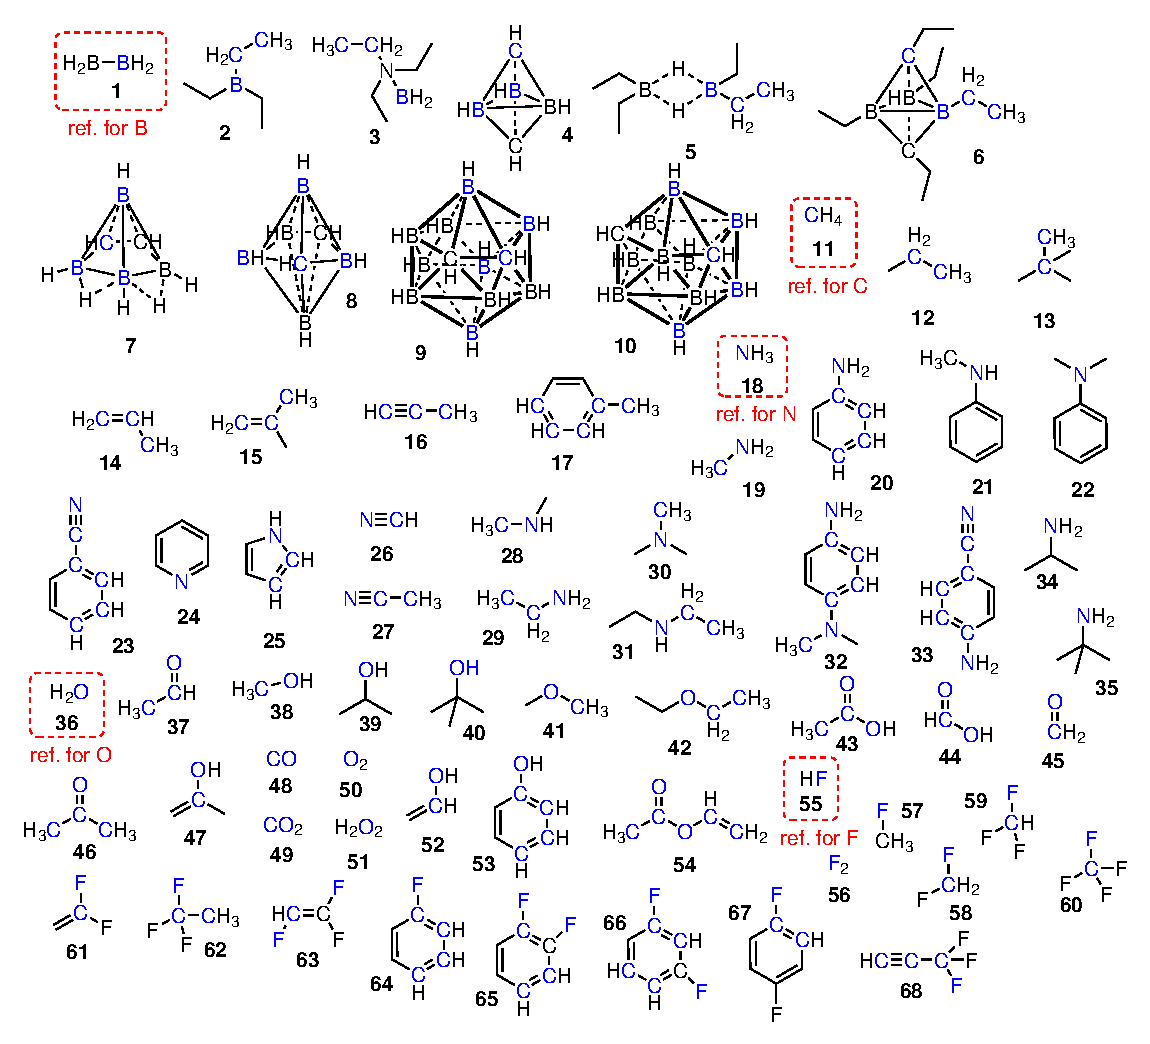
\includegraphics[width=\linewidth]{Figure3}
	\caption{Molecules for the benchmark \cite{pueyobellafontPredictingCoreLevel2017}. The atoms for which experimental BE are provided are highlighted in blue.  The reference compound used for each atom are highlighted in red.}
	\label{fig:core185}
\end{figure}

\paragraph{Binding energies of molecules grafted on surfaces.} Following the protocol established by Ebadi and co-workers \cite{ebadiInsightsLiMetalOrganic2019}, the binding energies (\dbe{}) of molecules adsorbed on surfaces were investigated. Initially, bulk Ca (from the Material Project, \texttt{MP-45}), CaO (\texttt{MP-2605}), and \ce{CaH2} (\texttt{MP-23713}) were selected, and their atomic positions and cell parameters were optimized.

Subsequently, to determine the optimal surface orientation, 1x1 slabs with increasing thickness along different low-index orientations [(100), (110), and (111)] were constructed using ASE \cite{larsenAtomicSimulationEnvironment2017}. The slabs were relaxed with the central two layers frozen to mimic bulk conditions, with the distance between slab repetitions set to 10 times the $c$ cell parameter of the bulk. For each orientation, the surface energy $\gamma^{hkl}$ was calculated by least-squares fitting of the following expression \cite{sunEfficientCreationConvergence2013,tranSurfaceEnergiesElemental2016}:
\begin{equation}
	E^{hkl}(N) = E_0\,N + 2A\,\gamma^{hkl} \label{eq:surf}
\end{equation}
where $N$ is the number of layers in the slab, $A$ is the slab surface area, $E^{hkl}(N)$ is the energy of the relaxed slab cut along $(hkl)$, and $E_0$ approximates the bulk energy. The results (Table \ref{tab:surf}, Fig.~\ref{fig:surf}) indicate that (100) surfaces are the most energetically favorable, consistent with findings in the literature \cite{deleeuwDensityFunctionalTheory2000,ebadiInsightsLiMetalOrganic2019}.

\begin{table}[!h]
	\centering
	\begin{tabular}{lccc}
		\toprule
		&	\ce{Ca} & \ce{CaO} &	\ce{CaH2} \\
		\midrule
		(100) & 0.555 ($N\in[6,16]$) & 0.470 ($N\in[6,16]$) & 0.871  ($N\in[12,32]$)\\
		(110) & 0.630  ($N\in[6,16]$)& 1.777  ($N\in[6,16]$)& 1.109 ($N\in[12,32]$)\\
		(111) & 0.563  ($N\in[6,16]$) & 4.080  ($N\in[5,15]$)  & 1.117   ($N\in[12,32]$) \\ 
		\bottomrule
	\end{tabular}
	\caption{Surface energies ($\gamma^{hkl}$, in \si{\joule\per\meter\squared}) of Ca, CaO, and \ce{CaH2} slabs along different orientations, as determined through Eq.~\eqref{eq:surf} using the $N$ values given in parentheses.}
	\label{tab:surf}
\end{table}

Using the (100) orientation, 3x3 slabs (consisting of 6 layers, with a vacuum of \SI{20}{\angstrom} between two slab repetitions) were created and relaxed (with frozen cell parameters). Additionally, following its documented favorability \cite{deleeuwDensityFunctionalTheory2000}, the adsorption of water on the CaO surface was investigated. An additional slab with full coverage (1 water molecule per surface Ca), denoted as \ce{CaO.H_2O}, was optimized. Compounds \textbf{a}-\textbf{i} (Fig.~\ref{fig:THFdegradation}) were subsequently introduced on both sides of the slab (initially approximately \SI{5}{\angstrom} away), followed by a final optimization (with frozen cell parameters). Finally, binding energies were computed for each relevant atom.

\section{Results}

\subsection{Biding energies in gas phase}

A comparison between experimental and computed \dbe\ is presented in Fig.~\ref{fig:xps_C185}. The agreement with previous investigations \cite{pueyobellafontPredictingCoreLevel2017,golzeAccurateAbsoluteRelative2020} shows that the SJ\textsuperscript{n} protocol provides reliable results for all atoms, with very small mean errors (<\SI{0.1}{\electronvolt}) and acceptable standard deviations (0.1 to \SI{0.4}{\electronvolt}). However, it should be noted that a reference per atom is necessary (Table \ref{tab:xpssjn}), as the difference between experimental and computed absolute BE increases with the atomic number. 
In contrast, the SJ protocol exhibits non-systematic errors, as indicated by the large standard deviations (>\SI{0.7}{\electronvolt}).


\begin{figure}[!h]
	\centering
	 \includegraphics[width=.8\linewidth]{Figure4}
	 \caption{Comparision between experimental and calculated gas phase \dbe{}, as computed with the SJ (blue) and SJ\textsubscript{n} (orange) protocols on the different atoms. For each of them, the error (as mean $\pm$ standard deviation) for both protocols is given.}
	 \label{fig:xps_C185}
\end{figure}

\begin{table}[!h]
	\centering
	\begin{tabular}{lcccc}
		\toprule
		& Reference & BE (exp.)  & BE (SJ\textsuperscript{n})  & $\Delta$(SJ\textsuperscript{n}- exp.)\\
		\midrule
		B1s & \ce{(BH2)2} & 196.50 & 201.47 & 4.97\\
		C1s & \ce{CH4} & 290.90 & 297.04 & 6.14\\
		N1s & \ce{NH3} & 405.60 & 413.58 & 7.98\\
		O1s & \ce{H2O} & 539.70 & 548.79 & 9.09\\
		F1s & \ce{HF} & 694.23 & 704.78 &10.55\\
		\bottomrule
	\end{tabular}
	\caption{Comparison between experimental (from Ref.~\cite{pueyobellafontPredictingCoreLevel2017}) and calculated (as computed with the SJ\textsuperscript{n} protocol) absolute BE.}
	\label{tab:xpssjn}
\end{table}

\clearpage
\subsection{Binding energies of slabs}

The impact of slab thickness on the resulting spectra is assessed in Fig.~\ref{fig:slabsthickness}. Increasing the slab thickness shifts the balance between surface and bulk features towards the latter, but it does not significantly change the peak positions. Therefore, further calculations can safely use the slabs with the fewest layers to save computation time. It should also be noted that the SJ\textsuperscript{n} protocol predicts a difference of \SI{7.6}{\electronvolt} between our reference (water, for oxygen) and the value of O1s in \ce{CaO}, which is close to the experimental value of \SI{7.8}{\electronvolt} \cite{cristHandbookMonochromaticXPS1999}. In contrast, the SJ protocol predicts a difference of only \SI{5}{\electronvolt}, further validating the use of the SJ\textsuperscript{n} protocol.


\begin{figure}[!h]
	\centering
	\includegraphics[width=\linewidth]{Figure5}
	\caption{Impact of the slab thickness (indicated as the number of layers) on the resulting XPS spectra (as computed with the SJ\textsuperscript{n} protocol).}
	\label{fig:slabsthickness}
\end{figure}

\clearpage
\bibliographystyle{unsrt}
\bibliography{biblio}

\clearpage
\appendix
\counterwithin{figure}{section}
\section{Appendix}
\begin{figure}[!h]
	\includegraphics[width=\linewidth]{FigureA1}
	\caption{Evolution of the surface energy for slabs of Ca, CaO, and \ce{CaH2} with increasing thickness ($N$) , as estimated by least-square fit of Eq.~\eqref{eq:surf}. For CaO, the surface energies of (110) and (111) are larger than \SI{1.25}{\joule\per\meter\squared}.}
	\label{fig:surf}
\end{figure}

\begin{figure}[!h]
	\centering
	\includegraphics[width=.8\linewidth]{FigureA2}
	\caption{Comparison between experimental and calculated gas phase \dbe{}, as computed with the SJ (blue) and SJ\textsubscript{n} (orange) protocols on the different atoms, and by shifting the BE by $E_F$ in Eq.~\eqref{eq:xpsbe}. For each of them, the error (as mean $\pm$ standard deviation) for both protocols is given.}
	\label{fig:xps_C185_fermi}
\end{figure}
	
\end{document}